\documentclass{article}

\usepackage{algorithm2e}
\usepackage{amsmath}
\usepackage{booktabs}
\usepackage[a4paper,textwidth=14cm, top=1cm, bottom=1cm,includehead,includefoot,
centering,footskip=1.5cm]{geometry}
\usepackage{graphicx}
\usepackage{hyperref}
% \usepackage{mathtools}
\usepackage{natbib}
\bibliographystyle{plainnat}

\hypersetup{
  colorlinks=true,
  linkcolor=blue,
  citecolor=blue,
  filecolor=blue,
  urlcolor=blue
}

\def\code#1{\texttt{#1}}

\title{A New Model-Based Notion of Variable Importance}
\date{}
\author{Author 1\\ Author 1 address \and Author 2\\Author 2 address}

\begin{document}

\maketitle


%%%%%%%%%%%%%%%%%%%%%%%%%%%%%%%%%%%%%%%%%%%%%%%%%%%%%%%%%%%%%%%%%%%%%%%%%%%%%%%%
% Abstract
%%%%%%%%%%%%%%%%%%%%%%%%%%%%%%%%%%%%%%%%%%%%%%%%%%%%%%%%%%%%%%%%%%%%%%%%%%%%%%%%
\begin{abstract}
Keep to 200 words or less and don't use references or mathematical markup.
\end{abstract}


%%%%%%%%%%%%%%%%%%%%%%%%%%%%%%%%%%%%%%%%%%%%%%%%%%%%%%%%%%%%%%%%%%%%%%%%%%%%%%%%
% Introduction
%%%%%%%%%%%%%%%%%%%%%%%%%%%%%%%%%%%%%%%%%%%%%%%%%%%%%%%%%%%%%%%%%%%%%%%%%%%%%%%%
\section{Introduction}

Talk about the improtance of extracting information from black-box models, blah, blah, blah.


\subsection{Variable importance metrics}

\subsubsection{Model-based approaches}
\begin{itemize}
  \item tree-based methods;
  \item linear and generalized linear models;
  \item MARS algorithm;
  \item Neural networks (specifically, the two approaches used later).
\end{itemize}

\subsubsection{Filter-based approaches}

% Currently lifted from ?caret::filterVarImp

For classification problems, the area under the ROC curve (AUC) is used as a measure of variable importance. For two class problems, a series a split points are chosen (not unlike a decision tree) for each predictor to predict each class and generate an ROC curve from which the AUC statistic is taken. For classification problems involving more than two classes, the problem is broken down into every possible one-vs-one problem, and the same procedure is applied. The maximum AUC for each variable is used as a measure of variable importance.

For regression, a parametric or nonparametric model is fit between each predictor and the outcome. For parametric models, some measure depending on the absolute value of the associated $t$-value is used as a measure of importance. Otherwise, the $R^2$ statistic is used.


\subsection{Partial dependence plots}

\citet{harrison-1978-hedonic} were among the first to analyze the well-known Boston housing data. One of their goals was to find a housing value equation using data on median home values from $n = 506$ census tracts in the suburbs of Boston from the 1970 census; see \citet[Table IV]{harrison-1978-hedonic} for a description of each variable. The data violate many classical assumptions like linearity, normality, and constant variance. Nonetheless, \citeauthor{harrison-1978-hedonic}---using a combination of transformations, significance testing, and grid searches---were able to find a reasonable fitting model ($R^2 = 0.81$). Part of the payoff for there time and efforts was an interpretable prediction equation which is reproduced in Equation~\eqref{eqn:boston}.
\begin{equation}
\label{eqn:boston}
\begin{aligned}
\widehat{\log\left(MV\right)} &= 9.76 + 0.0063 RM^2 + 8.98\times10^{-5} AGE - 0.19\log\left(DIS\right) + 0.096\log\left(RAD\right) \\
  & \quad - 4.20\times10^{-4} TAX - 0.031 PTRATIO + 0.36\left(B - 0.63\right)^2 - 0.37\log\left(LSTAT\right) \\
  & \quad - 0.012 CRIM + 8.03\times10^{-5} ZN + 2.41\times10^{-4} INDUS + 0.088 CHAS \\
  & \quad - 0.0064 NOX^2.
\end{aligned}
\end{equation}

Nowadays, many supervised learning algorithms can fit the data automatically in seconds---typically with higher accuracy. The downfall, however, is some loss of interpretation since these algorithms typically do not produce simple prediction formulas like Equation~\eqref{eqn:boston}. These models can still provide insight into the data, but it is not in the form of simple equations. For example, quantifying predictor importance has become an essential task in the analysis of "big data", and many supervised learning algorithms, like tree-based methods, can naturally assign variable importance scores to all of the predictors in the training data.

While determining predictor importance is a crucial task in any supervised learning problem, ranking variables is only part of the story and once a subset of "important" features is identified it is often necessary to assess the relationship between them (or subset thereof) and the response. This can be done in many ways, but in machine learning it is often accomplished by constructing \textit{partial dependence plots} (PDPs); see \citet{friedman-2001-greedy} for details. PDPs help visualize the relationship between a subset of the features (typically 1-3) and the response while accounting for the average effect of the other predictors in the model. They are particularly effective with black box models like random forests and support vector machines.

Let $\boldsymbol{x} = \left\{x_1, x_2, \dots, x_p\right\}$ represent the predictors in a model whose prediction function is $\widehat{f}\left(\boldsymbol{x}\right)$. If we partition $\boldsymbol{x}$ into an interest set, $\boldsymbol{z}_s$, and its compliment, $\boldsymbol{z}_c = \boldsymbol{x} \setminus \boldsymbol{z}_s$, then the "partial dependence" of the response on $\boldsymbol{z}_s$ is defined as
\begin{equation}
\label{eqn:avg_fun}
  f_s\left(\boldsymbol{z}_s\right) = E_{\boldsymbol{z}_c}\left[\widehat{f}\left(\boldsymbol{z}_s, \boldsymbol{z}_c\right)\right] = \int \widehat{f}\left(\boldsymbol{z}_s, \boldsymbol{z}_c\right)p_{c}\left(\boldsymbol{z}_c\right)d\boldsymbol{z}_c,
\end{equation}
where $p_{c}\left(\boldsymbol{z}_c\right)$ is the marginal probability density of $\boldsymbol{z}_c$: $p_{c}\left(\boldsymbol{z}_c\right) = \int p\left(\boldsymbol{x}\right)d\boldsymbol{z}_s$.
Equation~\eqref{eqn:avg_fun} can be estimated from a set of training data by
\begin{equation}
\label{eqn:pdf}
\bar{f}_s\left(\boldsymbol{z}_s\right) = \frac{1}{n}\sum_{i = 1}^n\widehat{f}\left(\boldsymbol{z}_s,\boldsymbol{z}_{i, c}\right),
\end{equation}
where $\boldsymbol{z}_{i, c}$ $\left(i = 1, 2, \dots, n\right)$ are the values of $\boldsymbol{z}_c$ that occur in the training sample; that is, we average out the effects of all the other predictors in the model.

Constructing a PDP \eqref{eqn:pdf} in practice is rather straightforward. To simplify, let $\boldsymbol{z}_s = x_1$ be the predictor variable of interest with unique values $\left\{x_{11}, x_{12}, \dots, x_{1k}\right\}$. The partial dependence of the response on $x_1$ can be constructed as follows:

\begin{algorithm}
\begin{enumerate}
  \item For $i \in \left\{1, 2, \dots, k\right\}$:
  \begin{enumerate}
    \item Copy the training data and replace the original values of $x_1$ with the constant $x_{1i}$.
    \item Compute the vector of predicted values from the modified copy of the training data.
    \item Compute the average prediction to obtain $\bar{f}_1\left(x_{1i}\right)$.
  \end{enumerate}
  \item Plot the pairs $\left\{x_{1i}, \bar{f}_1\left(x_{1i}\right)\right\}$ for $i = 1, 2, \dotsc, k$.
\end{enumerate}
\caption{A simple algorithm for constructing the partial dependence of the response on a single predictor $x_1$. \label{alg:pdp}}
\end{algorithm}
Algorithm~\ref{alg:pdp} can be quite computationally intensive since it involves $k$ passes over the training records. Fortunately, the algorithm can be parallelized quite easily (more on this in Section~\ref{sec:computational}). It can also be easily extended to larger subsets of two or more features as well.

For illustration, we will use a corrected version of the Boston housing data analyzed in \citet{harrison-1978-hedonic}; the data are available from Statlib at \url{http://lib.stat.cmu.edu/datasets/boston_corrected.txt}. Using the R package \texttt{randomForest} [REFERENCE], we fit a random forest with default tuning parameters and 500 trees. The model fit is reasonable, with an \textit{out-of-bag} (pseudo) $R^2$ of 0.89. The variable importance scores are displayed in Figure~\ref{fig:boston-rf-vip}. Both plots indicate that the percentage of lower status of the population (\code{lstat}) and the average number of rooms per dwelling (\code{rm}) are highly associated with the median value of owner-occupied homes (\code{cmedv}). They also indicate that the proportion of residential land zoned for lots over 25,000 sq.ft (\code{zn}) has little association with \code{cmedv}.
\begin{figure}[!htb]
  \label{boston-rf-vip}
  \centering
  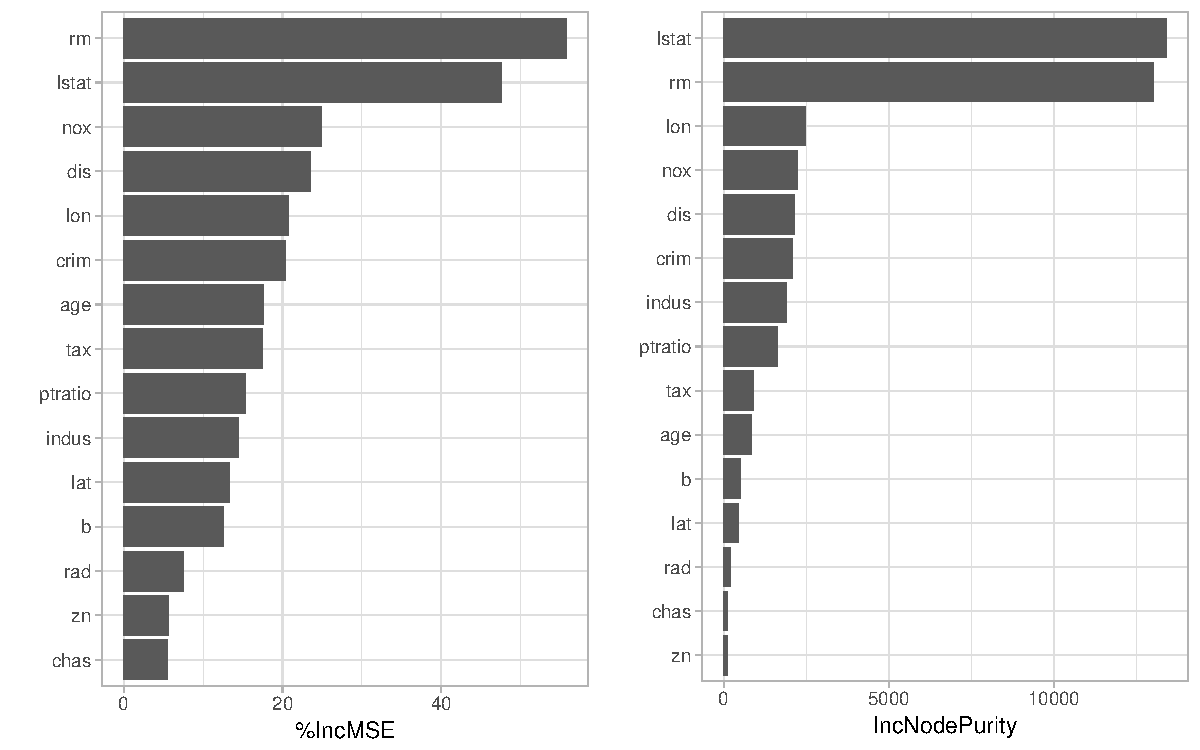
\includegraphics[width=1.0\textwidth]{boston-rf-vip}
  \caption{TBD.}
\end{figure}

The partial dependence functions for these three variables are displayed in Figure~\ref{fig:boston-rf-pdps}. Notice how the PDP for \code{zn} is essentially flat. It is this notion of "flatness" which we will use to define our variable importance measure.
\begin{figure}[!htb]
  \label{boston-rf-pdps}
  \centering
  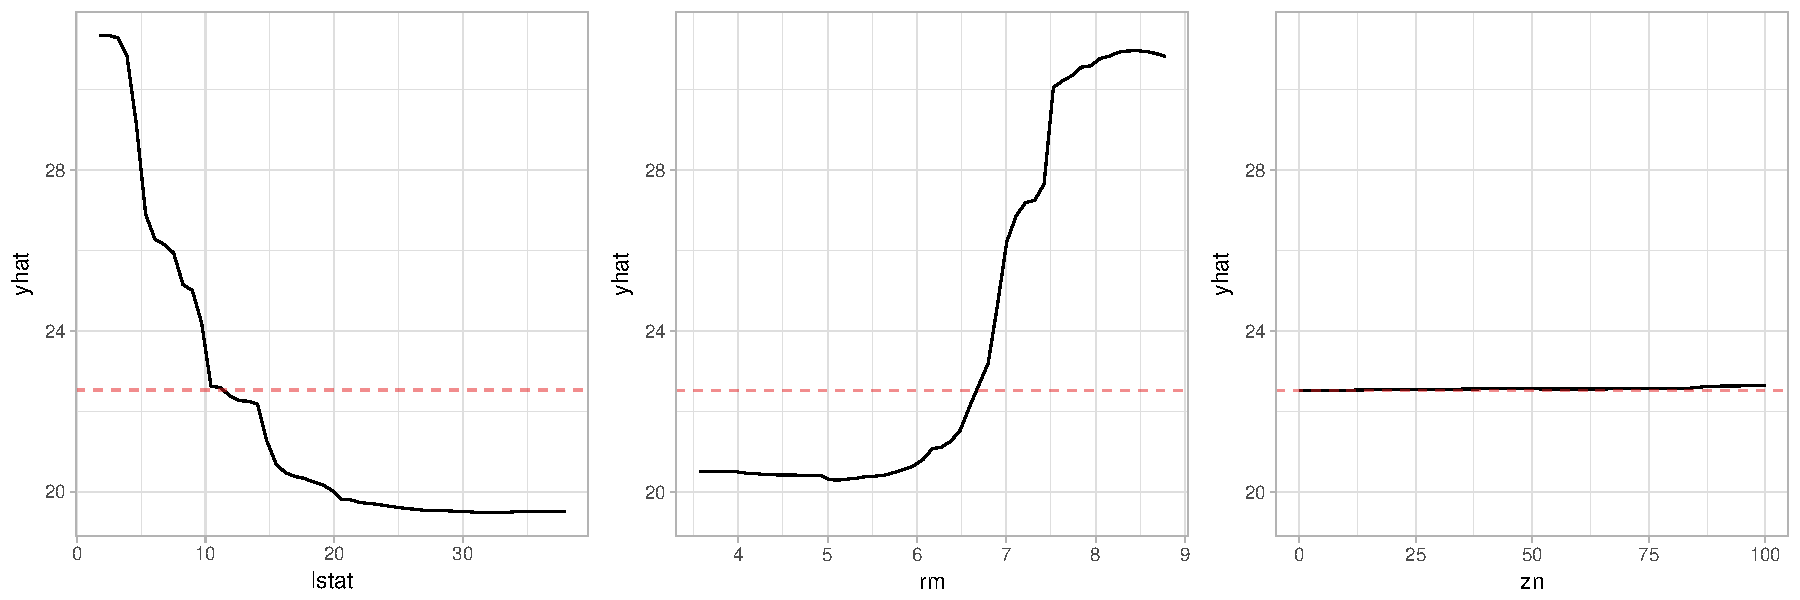
\includegraphics[width=1.0\textwidth]{boston-rf-pdps}
  \caption{TBD.}
\end{figure}


%%%%%%%%%%%%%%%%%%%%%%%%%%%%%%%%%%%%%%%%%%%%%%%%%%%%%%%%%%%%%%%%%%%%%%%%%%%%%%%%
% Prediction-based variable importance
%%%%%%%%%%%%%%%%%%%%%%%%%%%%%%%%%%%%%%%%%%%%%%%%%%%%%%%%%%%%%%%%%%%%%%%%%%%%%%%%
\section{Prediction-based variable importance}

Our notion of variable importance is based on any measure of the "flatness" of the partial dependence function. In general, we define
\begin{equation}
  imp\left(x\right) = flatness\left(\bar{f}_s\left(\boldsymbol{z}_s\right)\right),
\end{equation}
where $flatness$ is any measure of "flatness" of the curve. A simplle and effective measure to use is the range statistic. Based on Algorithm~\ref{alg:pdp}, our importance metric for predictor $x_1$ is simply
\begin{equation}
  imp\left(x_1\right) = \max_{i \in \left\{1, 2, \dots, k\right\}} \bar{f}_1\left(x_{1i}\right) - \min_{i \in \left\{1, 2, \dots, k\right\}} \bar{f}_1\left(x_{1i}\right).
\end{equation}


%%%%%%%%%%%%%%%%%%%%%%%%%%%%%%%%%%%%%%%%%%%%%%%%%%%%%%%%%%%%%%%%%%%%%%%%%%%%%%%%
% Examples
%%%%%%%%%%%%%%%%%%%%%%%%%%%%%%%%%%%%%%%%%%%%%%%%%%%%%%%%%%%%%%%%%%%%%%%%%%%%%%%%
\section{Examples: a simple function of ten variables}

For illustration, we use one of the regression problems described in Friedman (1991) and Breiman (1996). Inputs are 10 independent variables uniformly distributed on the interval $\left[0, 1\right]$; only 5 out of these 10 are actually used. Outputs are created according to the formula
\begin{equation}
\mathcal{Y} = 10 \sin\left(\pi x_1 x_2\right) + 20 \left(x_3 - 0.5\right) ^ 2 + 10 x_4 + 5 x_5 + \epsilon,
\end{equation}
where $\epsilon \sim \mathcal{N}\left(0, \sigma\right)$.


We fit a simple neural network with eight hidden units and a weight decay of 0.01. These parameters were chosen using 5-fold cross-validation to maximize the root mean squared error (RMSE). The network diagram is displayed in Figure~\ref{fig:network} below.
\begin{figure}[!htb]
  \label{network}
  \centering
  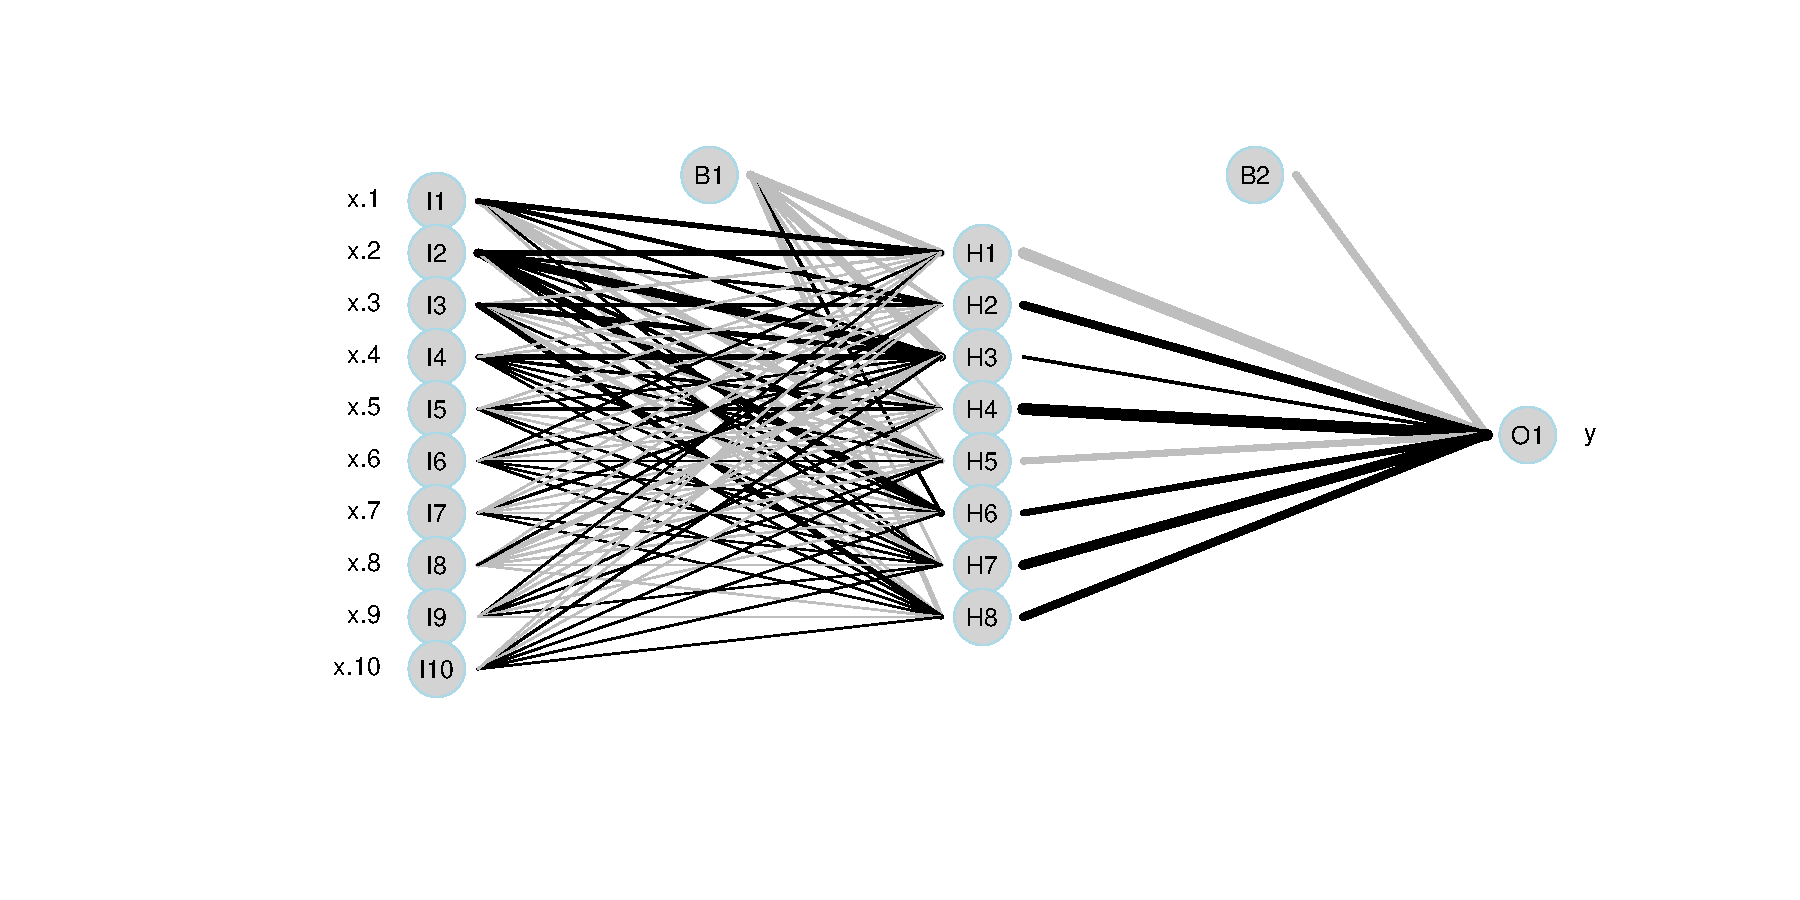
\includegraphics[width=1.0\textwidth]{network}
  \caption{Diagram of the neural network fitted to the Friedman 1 data set.}
\end{figure}

Variable importance plots are displayed in Figure~\ref{fig:network-vip}. Notice how the Garson and Olden algorithms incorrectly label some of the features not in the true model as "important".
\begin{figure}[!htb]
  \label{network-vip}
  \centering
  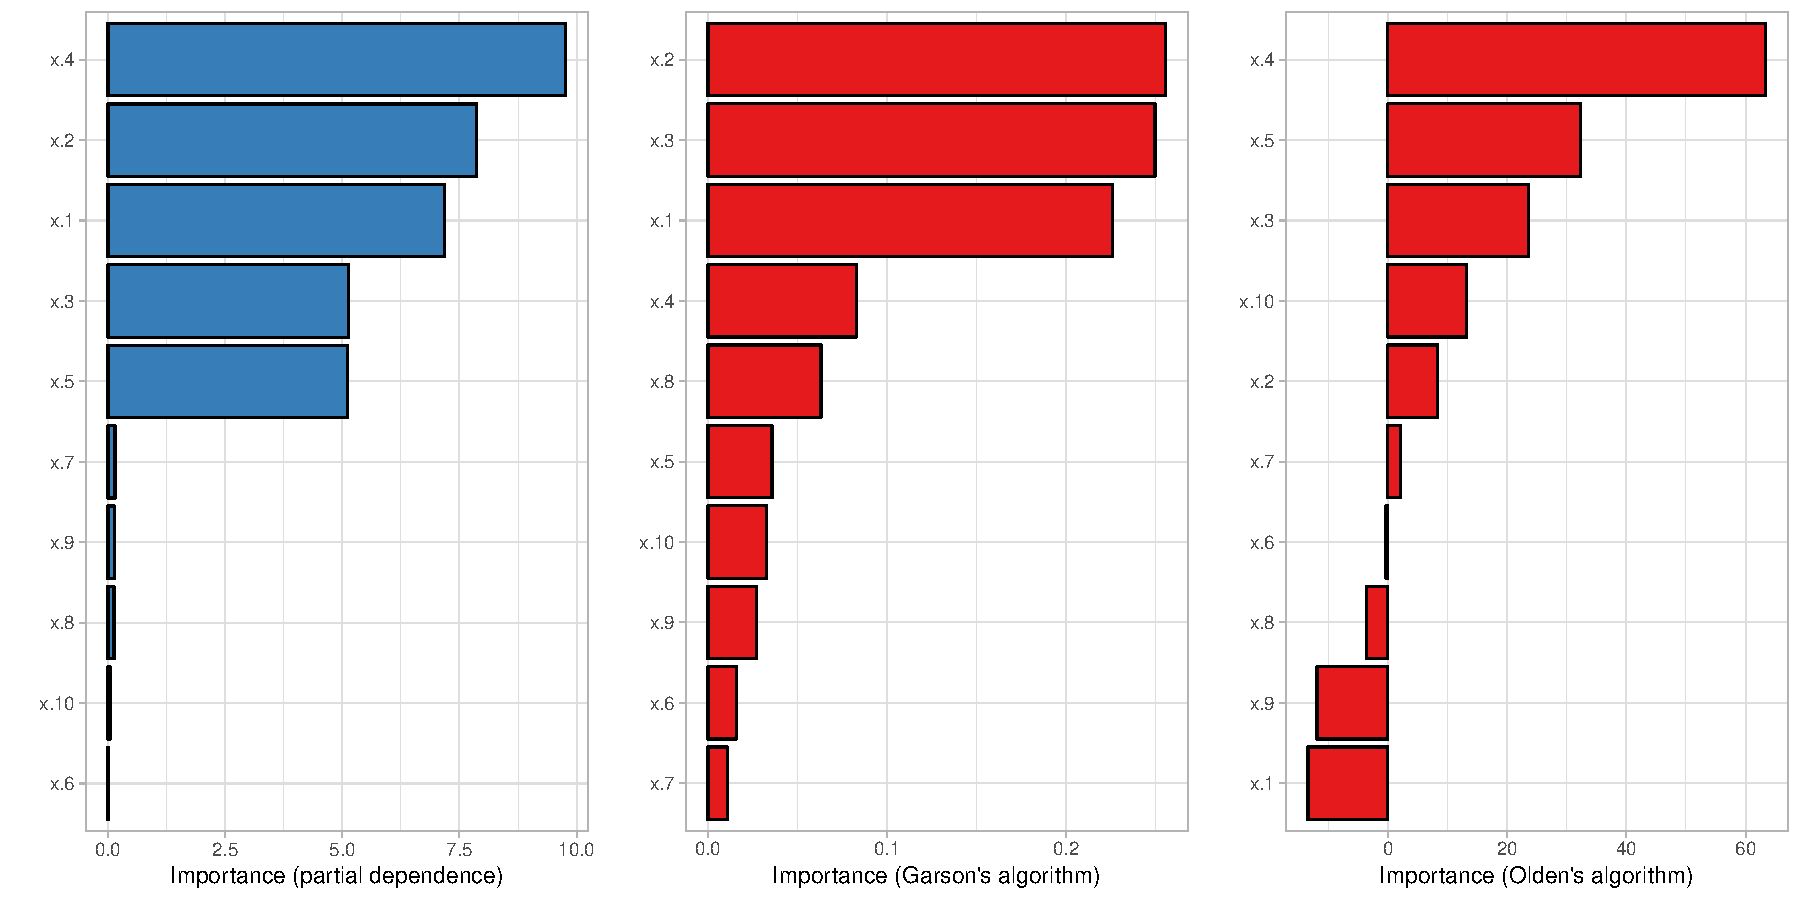
\includegraphics[width=1.0\textwidth]{network-vip}
  \caption{Variable importance plots for the neural network in Figure~\ref{fig:network}. \textit{Left}: partial dependence-based algorithm. \textit{Middle}: Garson's algorithm. \textit{Right}: Olden's algorithm.}
\end{figure}

For comparison, we fit a random forest [REFERENCE] with 1000 trees to the same data. Random forests (and other tree-based methods) have a natural way of denining variable importance. For details, see [REF]. Figure~\ref{fig:rf-vip} displays two types of importance measures obtained from the fitted random forest.


%%%%%%%%%%%%%%%%%%%%%%%%%%%%%%%%%%%%%%%%%%%%%%%%%%%%%%%%%%%%%%%%%%%%%%%%%%%%%%%%
% Discussion
%%%%%%%%%%%%%%%%%%%%%%%%%%%%%%%%%%%%%%%%%%%%%%%%%%%%%%%%%%%%%%%%%%%%%%%%%%%%%%%%
\section{Discussion}


%%%%%%%%%%%%%%%%%%%%%%%%%%%%%%%%%%%%%%%%%%%%%%%%%%%%%%%%%%%%%%%%%%%%%%%%%%%%%%%%
% Bibliography
%%%%%%%%%%%%%%%%%%%%%%%%%%%%%%%%%%%%%%%%%%%%%%%%%%%%%%%%%%%%%%%%%%%%%%%%%%%%%%%%
\bibliography{vip-methodology}

\end{document}
